\chapter{补充示例}

前三章给出了学位论文的官方要求。这里补充一些可能用到的示例。

\section{公式}

\subsection{带约束条件的公式}

假设一个数据集$D = {(x_i,y_i),i = 1,\dots,N}$,其中$(x_i,y_i)$是第$i$个标记示例,$x_i$是$M$维输入向量,$y_i\in\{+1,-1\}$是相关联的二进制标签,$N$是数据大小。形如$f(x)= w\cdot\Phi(x)+ b$的SVM分类器通过最大化边缘训练,等效为:
~\\
\begin{subequations}
\begin{align}
    \min_{w,b,\xi} \frac{1}{2}&\|w\|^2 + C\sum_{i=1}^N\xi_i\\
    \mathrm{s.t.}\quad &\forall i\in1,\dots,N:\xi_i\ge 0,y_i(w\cdot\Phi(x)+b)\ge 1-\xi_i
\end{align}
\label{eq:RT_SVMoptimizationFunction}
\end{subequations}
~\\
其中$\xi$是松弛变量,$C$是样本和边界间允许误差的权衡参数,$\Phi$是从原始输入空间到特征空间的映射。

\subsection{多等式}

MOSSE分别对分子和分母进行平均:
% ~\\
% \begin{equation}
% \begin{cases}
%     \hat{h}^\ast = \frac{A_t}{B_t}\\
%     A_t = \eta(\hat{y}_t\odot\hat{x}_t^\ast) + (1-\eta)A{t-1}\\
%     B_t = \eta(\hat{x}_t\odot\hat{x}_t^\ast) + (1-\eta)B{t-1}
% \end{cases}
% \label{eq:RT_MOSSEruningAverage}
% \end{equation}
% ~\\
% 其中$\eta$是学习率。这使得最近的帧更受重视,并且让先前帧的影响随时间呈指数级衰减。

\subsection{长公式}

目标的增强拉格朗日可以表示为:
~\\
\begin{equation}
\begin{aligned}
\mathcal{L}(\hat{g},h,\hat{\zeta})= &\frac{1}{2}\sum_{i=1}^N\|\hat{y}_i(j)-\mathrm{diag}(\hat{x}_i)^\top \hat{g}]\|_2^2 + \frac{\lambda}{2}\|h\|_2^2\\
                                    &+ \hat{\zeta}^\top(\hat{g}-\sqrt{D}FP^\top h)\\
                                    &+ \frac{\mu}{2}\|\hat{g}-\sqrt{D}FP^\top h\|_2^2
\end{aligned}
    \label{eq:CFwLB_augmented LagrangianObjectiveFunction}
\end{equation}
~\\

\subsection{矩阵}

令基础样本$x = (x_0,\dots,x_{n-1})$,循环矩阵$X$具有以下形式:
~\\
\begin{equation}
    X = C(x)= \begin{bmatrix}
        x_0&x_1&\dots&x_{n-1}\\
        x_{n-1}&x_0&\dots&x_{n-2}\\
        \vdots&\vdots&\ddots&\vdots\\
        x_1&x_2&\dots&x_0
        \end{bmatrix}
\label{eq:RT_circulantMatrix}
\end{equation}
~\\

\section{图}

\subsection{tikz画图}


在线Boosting算法流程如图\ref{fig:RF_onlineAdaboostFlowchart}所示。
~\\
\begin{figure}[htp]

\centering
\begin{tikzpicture}
\node[inner sep=0pt] (initialPosition) at (0,0)
    {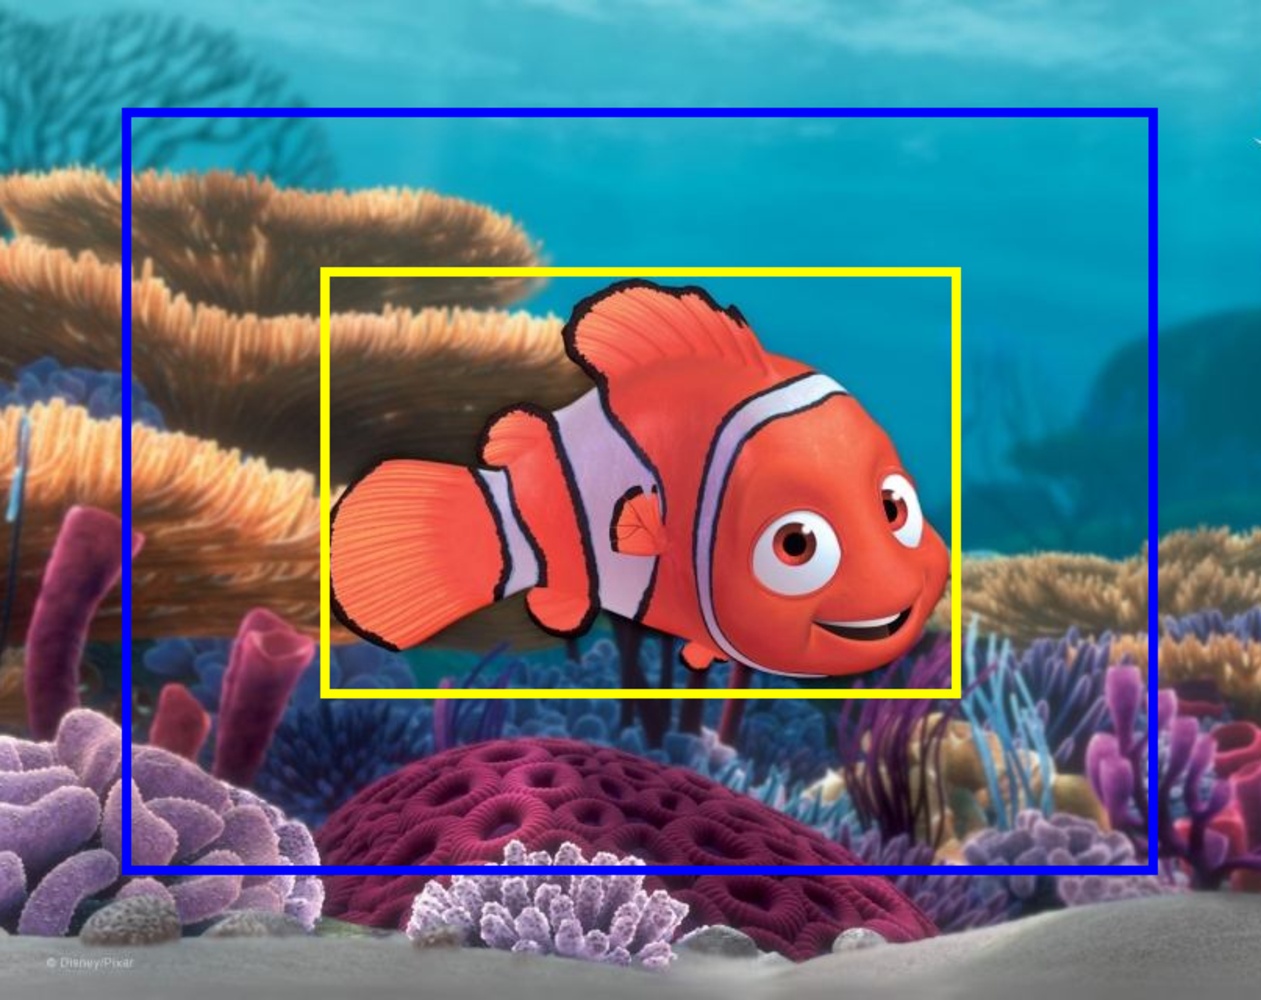
\includegraphics[width=.25\textwidth]{initialPosition.pdf}};
\node[inner sep=0pt] (sampleInSearchRegion) at (.4\textwidth,0)
    {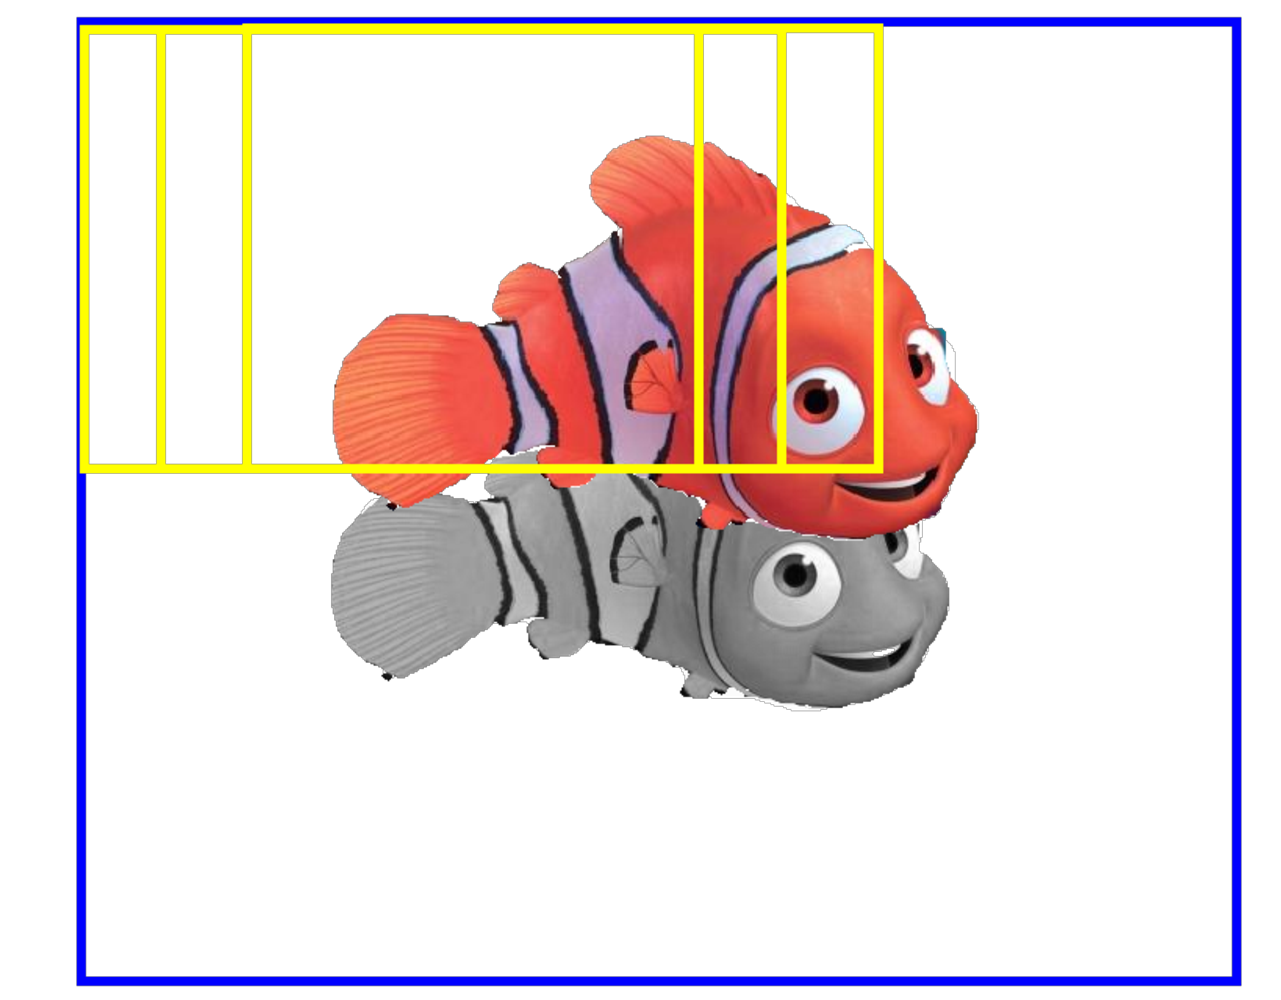
\includegraphics[width=.25\textwidth]{sampleInSearchRegion.pdf}};
\node[inner sep=0pt] (sampleArea) at (0,-0.3\textwidth)
    {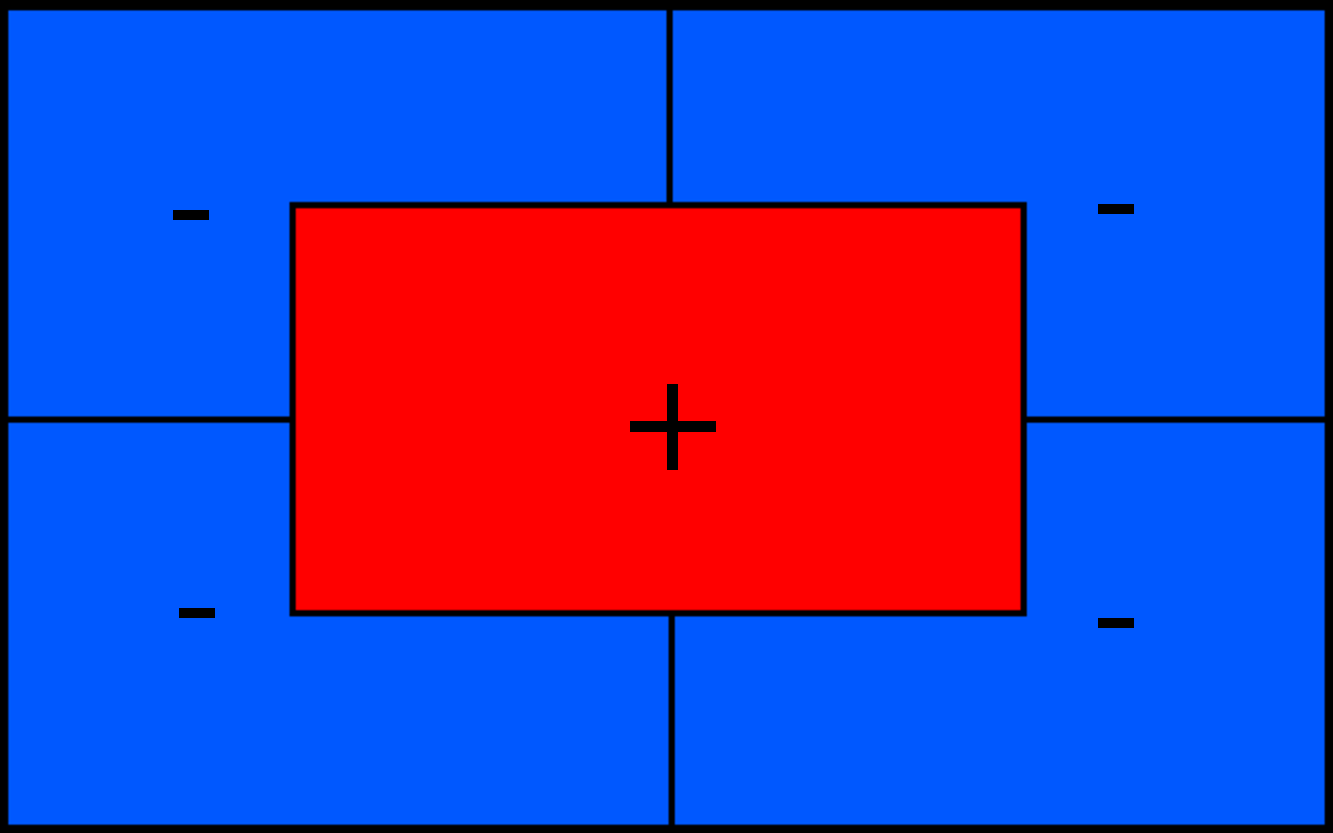
\includegraphics[width=.25\textwidth]{sampleArea.pdf}};
\node[inner sep=0pt] (confidenceMap) at (0.4\textwidth,-0.3\textwidth)
    {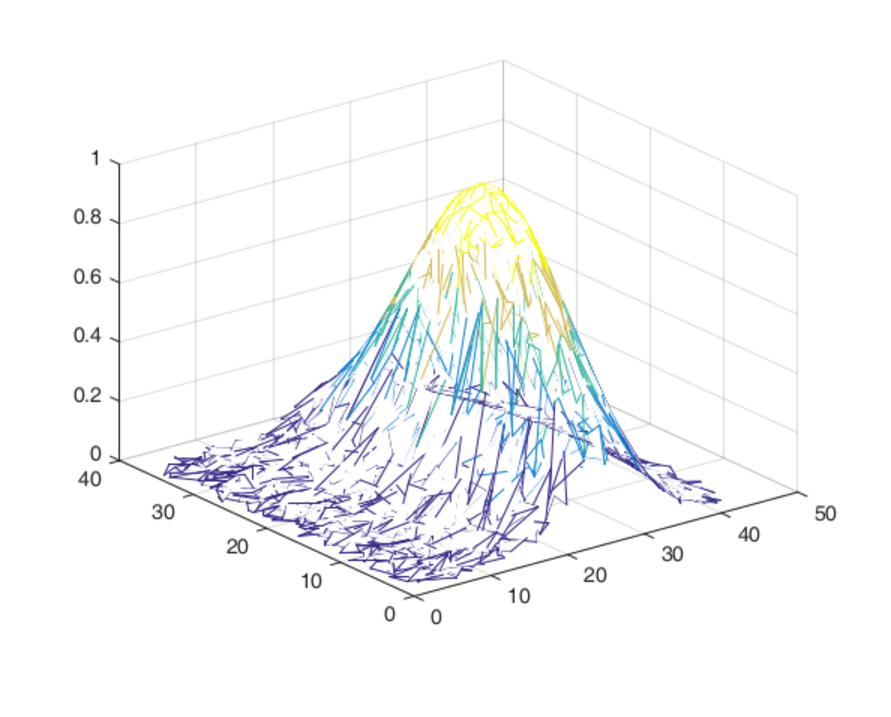
\includegraphics[width=.25\textwidth]{confidenceMap.pdf}};

\node[font=\small,align=left, above=1mm of initialPosition.north]{目标};
\node[font=\small,align=left, above=1mm of sampleInSearchRegion.north]{滑窗检测};
\node[font=\small,align=left, above=1mm of confidenceMap.north]{从置信图确\ 定目标位置};
\node[font=\small,align=left, above=1mm of sampleArea.north]{在新位置提取训练样本};
\draw[->,line width=1mm,blue] (initialPosition) -- (sampleInSearchRegion);
\draw[->,line width=1mm,blue] (sampleInSearchRegion) -- (confidenceMap.north);
\draw[->,line width=1mm,blue] (confidenceMap) -- (sampleArea);
\end{tikzpicture}
\caption{在线Boosting算法流程图}
\label{fig:RF_onlineAdaboostFlowchart}
\end{figure}

\subsection{多图排列}

跟踪过程中部分关键帧跟踪结果展示在图\ref{fig:LR_trackingResultSample}中。

\newcommand{\mycline}[1]{\tikz{\draw[#1 , line width=3] (0,0) -- (.5,0);}}
\begin{figure*}[htp]
	
	\centering
	\subfloat[Basketball]{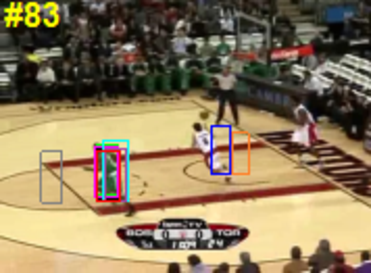
\includegraphics[width=0.31\linewidth,height=0.23\linewidth]{Figure2a1.pdf}
                       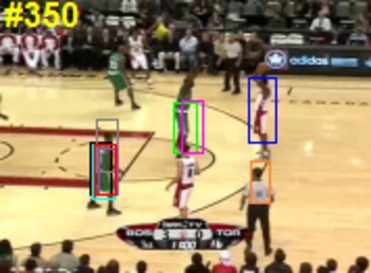
\includegraphics[width=0.31\linewidth,height=0.23\linewidth]{Figure2a2.pdf}
                       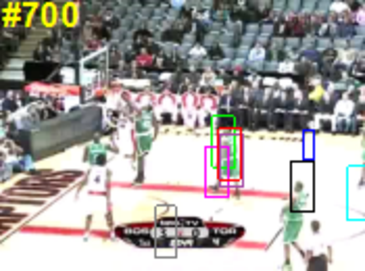
\includegraphics[width=0.31\linewidth,height=0.23\linewidth]{Figure2a3.pdf}
					   \label{fig:LR-Basketball}
					   }


	\centering
	\subfloat[David3]{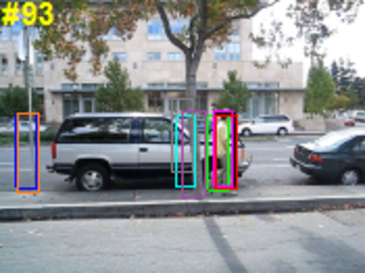
\includegraphics[width=0.31\linewidth,height=0.23\linewidth]{Figure2b1.pdf}
                      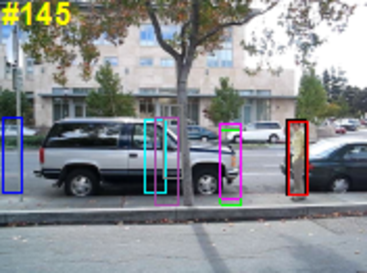
\includegraphics[width=0.31\linewidth,height=0.23\linewidth]{Figure2b2.pdf}
                      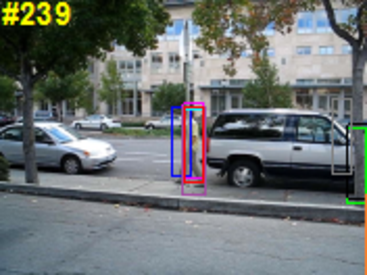
\includegraphics[width=0.31\linewidth,height=0.23\linewidth]{Figure2b3.pdf}
					  \label{fig:LR-David3}
					  }

	

	\centering
	\subfloat[Football]{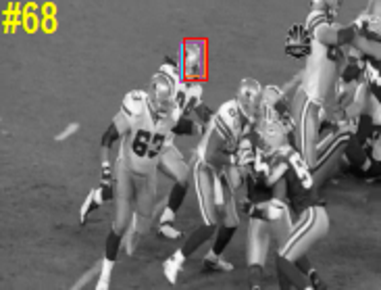
\includegraphics[width=0.31\linewidth,height=0.23\linewidth]{Figure2c1.pdf}
		                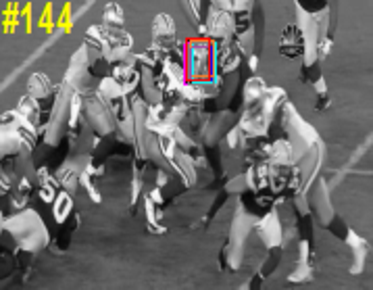
\includegraphics[width=0.31\linewidth,height=0.23\linewidth]{Figure2c2.pdf}
		                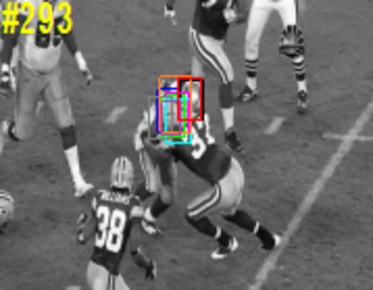
\includegraphics[width=0.31\linewidth,height=0.23\linewidth]{Figure2c3.pdf}
						\label{fig:LR-Football}
						}


	\centering
	\subfloat[Jogging]{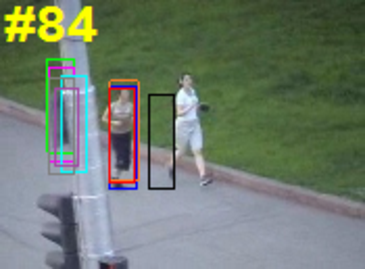
\includegraphics[width=0.31\linewidth,height=0.23\linewidth]{Figure2d1.pdf}
		               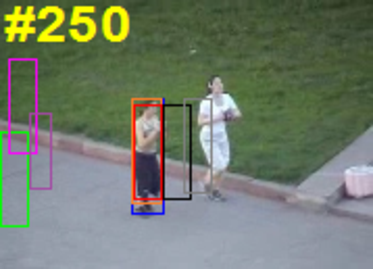
\includegraphics[width=0.31\linewidth,height=0.23\linewidth]{Figure2d2.pdf}
			           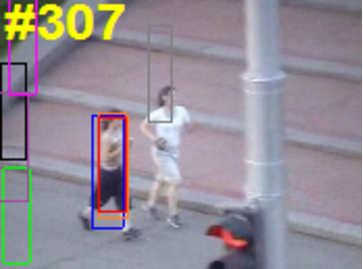
\includegraphics[width=0.31\linewidth,height=0.23\linewidth]{Figure2d3.pdf}
					   \label{fig:LR-Jogging}
					   }

		
	\centering
	\subfloat[Liquor]{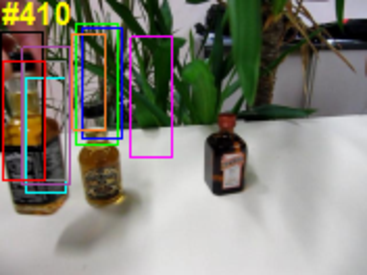
\includegraphics[width=0.31\linewidth,height=0.23\linewidth]{Figure2e1.pdf}
			          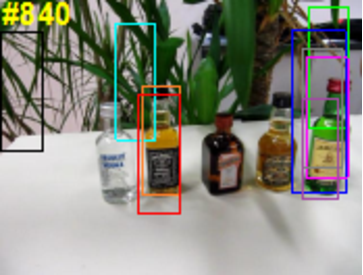
\includegraphics[width=0.31\linewidth,height=0.23\linewidth]{Figure2e2.pdf}
			          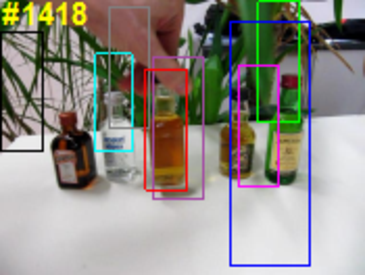
\includegraphics[width=0.31\linewidth,height=0.23\linewidth]{Figure2e3.pdf}
					  \label{fig:LR-Liquor}
					  }	

   \mycline{green}CT
   \mycline{blue}CXT
   \mycline{black}DT
   \mycline{pink}MIL
   \mycline{cyan}SCM
   \mycline{gray}Struck
   \mycline{orange}TLD
   \mycline{purple}VTD
   \mycline{red}Ours
   ~\\~\\
	\caption{跟踪过程中代表性序列帧及对比算法跟踪结果}
	\label{fig:LR_trackingResultSample}
\end{figure*}

\section{表格}

表\ref{tab:CFwLB_precision}展示了8种算法的20个像素偏差内的准确率。
~\\
\begin{table*}[htbp]
\centering
\renewcommand{\arraystretch}{1.5}
\zihao{5}\caption{8种算法20个像素偏差内的准确率}
    \begin{tabular}{|c|c|c|c|c|c|c|c|c|}
        \hline
        序列  & Frag  &  OAB  &  SBT  &  MIL  & Struck & CSK   & CFwLB   &  Ours \\ \hline

        Coke      & 0.034 & 0.168 & 0.048  & 0.117 & \textcolor{blue}{0.942} & 0.739 & 0.918   & \textcolor{red}{0.959}  \\ \hline
        David     & 0.121 & 0.151 & 0.204  & 0.229 & \textcolor{blue}{0.236} & \textcolor{blue}{0.236} & 0.144   & \textcolor{red}{0.396} \\ \hline
        Dog       & 0.173 & 0.157 & 0.079  & 0.197 & 0.157 & 0.144 & \textcolor{blue}{0.858}   & \textcolor{red}{0.992}  \\ \hline
        Doll      & 0.663 & 0.663 & 0.149  & 0.433 & 0.688 & 0.218 & \textcolor{blue}{0.947}& \textcolor{red}{ 0.986} \\ \hline
        Gym       & \textcolor{blue}{0.369} & 0.016 & 0.046  & 0.329 & 0.219 & 0.091 & 0.113   & \textcolor{red}{0.801}  \\ \hline
        KiteSurf  & 0.143 & 0.381 & 0.369  & 0.381 & \textcolor{blue}{0.905} & 0.321 & 0.274   & \textcolor{red}{0.964}  \\ \hline
        Surfer    & 0.176 & 0.045 & 0.133  & 0.088 & 0.157 & 0.005  & \textcolor{blue}{0.468}   & \textcolor{red}{0.997}  \\ \hline
    Sylvester     & 0.685 & 0.680 & 0.430  & 0.546 & \textcolor{blue}{0.929} & 0.717 & 0.921 & \textcolor{red}{0.947}\\ \hline
        Vase      & 0.166 & 0.155 & 0.129  & 0.166 & 0.140 & 0.166  & \textcolor{blue}{0.181}   & \textcolor{red}{0.657}  \\ \hline \hline

        平均      &0.281  & 0.268 & 0.176  & 0.276 & 0.486 & 0.293  & \textcolor{blue}{0.536}& \textcolor{red}{0.855} \\ \hline
\end{tabular}
\label{tab:CFwLB_precision}
\end{table*}
\zihao{-4}\setlength{\baselineskip}{20pt}


\section{文献引用}

Li等\cite{li2007robust}人采用三维时域张量子空间学习进行视觉跟踪。文献\citens{wen2009incremental}中,通过基于加权张量子空间(Weighted Tensor Subspace, WTS)的增量学习算法来适应跟踪期间的外观变化。

通常的做法是稀疏取样,即每帧只随机选取若干样本\cite{Zhang2012Real,kalal2012tracking,babenko2011robust,saffari2009line,hare2016struck}。

中文文献引用测试\cite{yuanaiping2014}。

